\documentclass[reqno]{amsart}

\usepackage{amsfonts,latexsym,amsthm,amssymb,amsmath,amscd,euscript,bm}
\usepackage[sc]{mathpazo}
\usepackage[margin = 2.6cm]{geometry}
\usepackage{enumitem}
\usepackage{hyperref}
\usepackage{graphicx}
% sets numbering of enumerate to a, b, c, ...
\renewcommand{\theenumi}{\alph{enumi}}

% Theorems, propositions, etc.
\newtheorem{theorem}{Theorem}
\newtheorem{proposition}[theorem]{Proposition}
\newtheorem{lemma}[theorem]{Lemma}
\newtheorem{corollary}[theorem]{Corollary}

\theoremstyle{definition}
\newtheorem{definition}[theorem]{Definition}
\newtheorem*{claim}{Claim}

\theoremstyle{remark}
\newtheorem*{remark}{Remark}
\newtheorem*{notation}{Notation}


% Math blackboard font
\newcommand{\nc}{\newcommand}
\nc{\on}[1]{\operatorname{#1}}

\nc{\R}{\mathbb R}
\nc{\C}{\mathbb C}
\nc{\Q}{\mathbb Q}
\nc{\Z}{\mathbb Z}
\nc{\N}{\mathbb N}
\nc{\HH}{\mathbb H}
\nc{\DD}{\mathbb D}
\nc{\TT}{\mathbb T}
\nc{\EE}{\mathbb E}
\nc{\PP}{\mathbb P}

\nc{\cT}{\mathcal T}
\nc{\cA}{\mathcal A}
\nc{\cM}{\mathcal M}
\nc{\cR}{\mathcal R}
\nc{\cB}{\mathcal B}
\nc{\cG}{\mathcal G}
\nc{\cD}{\mathcal D}
\nc{\cS}{\mathcal S}
\nc{\cF}{\mathcal F}
\nc{\cL}{\mathcal L}
\nc{\cE}{\mathcal E}

\nc{\diam}{\operatorname{diam}}
\nc{\supp}{\operatorname{supp}}
\nc{\loc}{\text{loc}}

% Why the f*** would you ever use \epsilon
\renewcommand{\epsilon}{\varepsilon}
\renewcommand{\emph}{\textsc}
\renewcommand{\Re}{\operatorname{Re}}
\renewcommand{\Im}{\operatorname{Im}}

\let\vec\mathbf

% Title: change problem set number as needed
\title
{
	\emph{Maximal functions}
} 

\author{Jason Zhao}
\date{\today}

\begin{document}
\maketitle

\begin{abstract}
	Given a family of linear operators $\{T_t\}_{t > 0}$ and $f \in L^p (\R^d)$, we are interested in finding the conditions under which the convergence $T_t f \to f$ holds pointwise almost everywhere. Typically one knows that pointwise convergence holds for a dense subclass of ``nice'' functions, such as test functions $f \in C^\infty_c (\R^d)$ or Schwartz functions $f \in \cS(\R^d)$. We would like to pass this result to the limit uniformly in $t$ to extend it to $f \in L^p (\R^d)$. This motivates the analysis of the maximal operator 
		\[ T^* f(x) := \sup_t |T_t f(x)|, \]
	and the study of its boundedness on $L^p (\R^d)$. Applications include the ergodic theorem (dynamical systems), the classical Dirichlet problem (PDE), and pointwise a.e. convergence of Fourier series (classical Fourier analysis). These notes draw from \cite{Duoandikoetxea2001} and \cite{Stein1993}. 
\end{abstract}

\tableofcontents

\section{Approximation to the identity}

Let $\phi \in L^1 (\R^d)$ such that $\int \phi = 1$, then define
	\[ \phi_t (x) := \frac{1}{t^d} \phi(x/t). \]
We say that the family $\{ \phi_t  \}_{t > 0}$ forms an \emph{approximation of the identity}. The name comes from the convergence of the family to the Dirac measure at the origin $\delta_0$ in the sense of tempered distributions: for any $f\in \cS$, it follows from a change of variables and the dominated convergence theorem that
	\[ \lim_{t \to 0} \langle \phi_t, f \rangle = \lim_{t \to 0} \int_{\R^d} \frac{1}{t^d} \phi(t/x) f(x) \, dx =  \lim_{t \to 0}\int_{\R^d} \phi(x) f(tx) \, dx = g(0) = \langle \delta_0, g \rangle.  \]
Since the Dirac measure furnishes the identity with respect to the convolution operation, we further have
	\[ \lim_{t \to 0} (\phi_t * f)(x) = f(x) \]	
for any $f \in \cS$ and $x \in \R^d$. We will consider the following question: in what sense does the convergence $\phi_t * f \to f$ hold, and under what conditions? In particular, we are interested in pointwise convergence and convergence in $L^p (\R^d)$. The latter is immediate;

\begin{theorem}
	Let $1 \leq p < \infty$ and suppose $\{ \phi_t\}_t$ forms an approximation of the identity, then 
		\[ \lim_{t \to 0} ||\phi_t * f - f||_{L^p} = 0 \]
	for $f \in L^p (\R^d)$. The convergence holds in the endpoint case $p = \infty$ when $f \in C_0 (\R^d)$.
\end{theorem}

\begin{proof}
	Using $\int \phi = 1$ and a change of variables, we can write
		\[ (\phi_t * f)(x) - f(x) = \int_{\R^n} \phi(y) (f(x - ty) - f(x)) \, dy. \]
	Taking the $L^p$-norm and applying Minkowski's integral inequality to the right, we obtain	
		\[ ||\phi_t * f - f||_{L^p} \leq \int_{\R^n} |\phi(y)| \, ||f (x - ty) - f(x)||_{L^p_x} \, dy. \]
	We need to exploit smallness of the $L^1$-norm of $\phi$ outside a large radius along with smallness of the $L^p$-norm for $|ty| \ll 1$. For the latter, it follows from the dominated convergence theorem in the case $1 \leq p < \infty$ or uniform continuity in the case $p = \infty$ that for every $\epsilon > 0$ we can choose $\delta > 0$ such that 
		\[ || f (x + h) - f(x)||_{L^p_x} < \frac{\epsilon}{2 ||\phi||_{L^1}} \]
	whenever $|h| < \delta$. To control the former, choose $t \ll 1$ such that
		\[ \int_{|y| > \delta/t} |\phi(y)| \, dy < \frac{\epsilon}{4 ||f||_{L^p}}. \]
	We conclude
		\begin{align*}
			 ||\phi_t * f - f||_{L^p}
			 	&\leq
			 	\left( \int_{|y| \geq \delta/t} + \int_{|y| < \delta/t}\right) |\phi(y)| \, ||f (x - ty) - f(x)||_{L^p_x} \, dy\\
			 &	\leq 2|| f||_{L^p} \int_{|y| > \delta/t} |\phi(y)| \, dy + \frac{\epsilon}{2 ||\phi||_{L^1}} \int_{|y| < \delta/t} |\phi(y)| \, dy < \epsilon.
		\end{align*}
\end{proof}

As a consequence, we know that there exists a sequence $t_k \to 0$ such that 
		\[ \lim_{k \to \infty} (\phi_{t_k} * f)(x) = f(x) \]
	for a.e. $x \in \R^d$. Hence if the limit of $\phi_t * f$ exists pointwise, then it must equal $f$ a.e. However, $f \in L^p (\R^d)$ is far from sufficient for establishing pointwise convergence. We do however know that the result holds Schwartz functions $f \in \cS$, which form a dense subspace of $L^p (\R^d)$ for $1 \leq p < \infty$ and $C_0 (\R^d)$ for the endpoint $p = \infty$. Therefore, it suffices to show that the set of functions $f \in L^p (\R^d)$ such that $\phi_t * f \to f$ pointwise a.e. forms a closed subspace of $L^p (\R^d)$. It turns out that this is closely related to establishing a weak-type $(p, q)$ bound for the corresponding \emph{maximal operator} defined as	
	\[ M_\phi f (x) := \sup_{t > 0} |(\phi_t * f) (x)|. \]
More generally, we have the following theorem:


\begin{theorem}
	Let $(X, \mu)$ be a measure space and $\{ T_t \}_{t > 0}$ be a family of linear operators on $L^p (X, \mu)$. Suppose that the corresponding \emph{maximal operator}
		\[ T^* f (x) := \sup_{t > 0} |T_t f(x)| \]
	is weak-type $(p, q)$ for exponents $1 \leq p \leq \infty$ and $1 \leq q < \infty$, then the set
		\[ \{ f \in L^p (X, \mu) : \lim_{t \to 0} T_t f(x) = f(x) \text{ a.e.} \} \]
	is closed in $L^p (X, \mu)$. \label{thm:approxidentity}
\end{theorem}

\begin{proof}
	Let $\{ f_n \}_n$ be a sequence of functions converging to $f \in L^p (X, \mu)$ in norm and such that $T_t f_n \to f_n$ pointwise a.e., we want to show that $T_t f  \to f$ pointwise a.e. For $x \in X$ such that $T_t f_n (x) \to f_n (x)$, it follows from the triangle inequality that 
		\[ \limsup_{t \to 0} |T_t f(x) - f(x)| \leq \limsup_{t \to 0} |T_t (f - f_n) (x) - (f - f_n)(x)| \leq T^* (f - f_n)(x) + |(f - f_n)(x)|. \]
	It follows that
		\begin{align*}
			\mu \{ x \in X :  \limsup_{t \to 0} |T_t f(x) - f(x)| > \lambda \}
				&\leq \mu \{ x \in X : T^* (f - f_n)(x) > \lambda/2\} +  \mu\{ x \in X : |(f - f_n) (x)| > \lambda/2 \} \\
				&\leq \left( \frac{2C}{\lambda} ||f - f_n||_{L^p} \right)^q + \left( \frac2\lambda ||f - f_n||_{L^p} \right)^p \overset{n \to \infty}{\longrightarrow} 0,
		\end{align*}
	 where in the first inequality we use sub-additivity of the measure $\mu$, and in the second inequality we apply the weak-type $(p, q)$-inequality and Chebyshev's inequality. As this holds for all $\lambda > 0$, we can write
	 	\[ \mu \{ x \in X : \limsup_{t \to 0} |T_t f(x) - f(x)| > 0 \} \leq \sum_{k = 1}^\infty  \mu \{ x \in \R^d : \limsup_{t \to 0} |T_t f(x) - f(x)| > 1/k \} = 0, \]
	 which shows $T_t f(x) \to f(x)$ for a.e. $x \in \R^d$, as desired. 
\end{proof}




\subsection{One-sided maximal function}

Let $f \in L^1_{\loc} (\R)$, then the \emph{one-sided Hardy-Littlewood maximal function} of $f$ is defined by
	\[ Mf (x) := \sup_{h > 0} \frac1h \int_{x}^{x + h} |f (t)| dt. \]
The operator $M$ is known as the one-sided Hardy-Littlewood maximal operator. It is clear that the operator is sub-linear, and it follows from the dominated convergence theorem that the averaging operator
	\[ A_h f(x) := \frac1h \int_x^{x + h} |f(t)| dt \]
is continuous. As the maximal operator is defined pointwise as the supremum of the averaging operators indexed by $h > 0$, it follows that $Mf$ is lower semi-continuous. Thus we can view the maximal operator as a ``smoothing'' operator, allowing us to make quantitative comparisons between pointwise values of a generic function. Furthermore it controls the approximation to the identity formed by the step function $\phi := \mathbb 1_{[0, 1]}$, so in view of Theorem \ref{thm:approxidentity}, we aim to show a weak-type $(p, q)$-inequality to conclude the classical Lebesgue differentiation theorem;

\begin{theorem}[Lebesgue differentiation theorem]
	Let $f \in L^1_{\loc} (\R)$, then 
		\[ f(x) = \lim_{h \to 0} \frac1h \int_x^{x + h} f(t) \, dt \]
	for a.e. $x \in \R$. 
\end{theorem}
	
Points where the Lebesgue differentiation theorem hold are known as \emph{Lebesgue points}. Dimensional analysis shows that no weak-type $(p, q)$ inequality can hold in the off-diagonal case $p \neq q$. Indeed, for $\alpha > 0$, set $f_\alpha (x) := f(x/\alpha)$. Then by a change of variables, 
	\[ Mf_\alpha (x) = \sup_{h > 0} \frac1h \int_x^{x + h} |f(t/\alpha)| \, dt = \sup_{h > 0} \frac{\alpha}{h}\int_{x/\alpha}^{x/\alpha + h/\alpha} |f(t)| \, dt = \sup_{h > 0} \frac1h \int_{x/\alpha}^{x/\alpha + h} |f(t)| \, dt = Mf (x/\alpha) \]
and
	\[ ||f_\alpha||_{L^p} = \left( \int_\R f(t/\alpha) \, dt \right)^{1/p} = \alpha^{1/p} ||f||_{L^p}. \]
Therefore a weak-type $(p, q)$ inequality applied to $f_\alpha$ gives
	\[ \alpha^{1/q} || Mf ||_{L^{q,\infty}} \lesssim \alpha^{1/p} ||f||_{L^p}, \]
where the bound can only hold uniformly provided that $p = q$. We will give the original proof of the weak-type $(1, 1)$ inequality due to F. Riesz in \cite{Riesz1932}, relying on a precursor of the Calderon-Zygmund decomposition;

\begin{lemma}[Rising sun lemma]
	Let $F : [a,b] \to \R$ be continuous and let $A \subseteq (a, b)$ be the set of $x \in (a, b)$ such that there exists $y \in (x, b)$ satisfying $F(y) >F(x)$. Then there exists an at most countable collection of disjoint open intervals $\{(a_k, b_k)\}_k$ such that 
		\[  A = \bigcup_k (a_k, b_k), \qquad F(a_k) \leq F(b_k). \]	
\end{lemma}

\begin{figure}[h]
	\begin{center}
		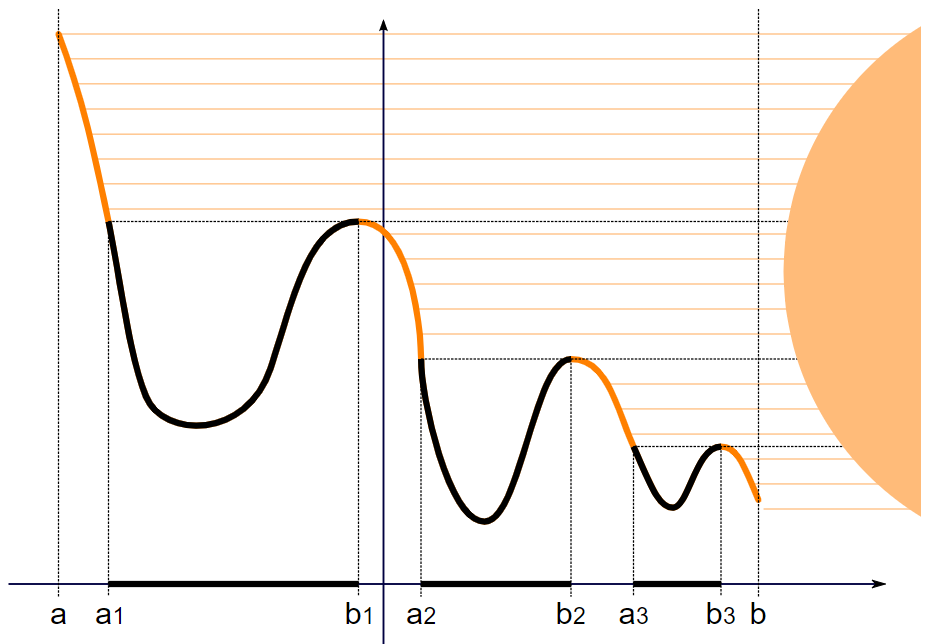
\includegraphics[scale = 0.4]{risingsun}
	\end{center}
	\caption{The points $b_k$ form the ``peaks'' of the ``hills'' casting ``shadows'' on the region $(a_k, b_k)$ as the ``sun rises''.}
\end{figure}

\begin{proof}
	It is clear by definition and continuity that $A$ is open, so, assuming it is non-empty, we know that it takes the form of an at most countable disjoint union of open intervals. It remains to verify $F(a_k) \leq F(b_k)$. Assume otherwise, i.e. $F(a_k) >F(b_k)$. By the extreme value theorem, we can find $x \in [a_k, b_k)$ satisfying
		\[ F(x) = \max_{y \in [a_k, b_k]} F(y). \]
	If $x > a_k$, then by definition of $A$ we know $F(y) > F(x)$ for some $y \in (x, b)$. It follows that
		\[ F(b_k) < F(a_k) \leq F(x) < f(y). \]
	We claim that $y \in (b_k, b)$, which by definition implies $b_k \in A$, a contradiction. Indeed, if the claim fails, then $y \in [a_k, b_k]$, contradicting the choice of $x$ as maximising $f$ on $[a_k, b_k]$. This completes the proof. 
\end{proof}

\begin{theorem}[One-sided Hardy-Littlewood maximal inequality]
	Let $f \in L^1 (\R)$, then 
		\[ |\{ x \in \R : Mf (x) > \lambda \}| \leq \frac1\lambda \int_{Mf > \lambda} |f(t)| \, dt. \]	
	In particular, the maximal operator is weak-type $(1, 1)$ and strong-type $(p, p)$ for $1 < p \leq \infty$.	
\end{theorem}

\begin{proof}
	The strong-type $(\infty, \infty)$ inequality is clear, so Marcinkiewicz interpolation furnishes the strong-type $(p, p)$ inequalities for $1 < p \leq \infty$ provided we show the weak-type $(1, 1)$-inequality. We argue using the rising sun lemma, letting $F: \R \to \R$ be the continuous function
		\[ F(x) := \int_{-\infty}^x |f(t)| \, dt - \lambda x. \]
	Observe that $Mf (x) > \lambda$ if and only if there exists $h > 0$ such that $F(x + h) - F(x) > 0$. This allows us to write the super-level set $Mf(x) > \lambda$ as an ascending union of sets $A_k \subseteq [-k, k]$ given by 
		\begin{align*}
			 \{ x \in \R : Mf(x) > \lambda \} 
			 	&= \{ x \in \R : F(y) > F(x) \text{ for some $y \in (x, \infty)$} \} \\
			 	&= \bigcup_{k \in \N} \{ x \in [-k, k] : F(y) > F(x) \text{ for some $y \in (x, k)$}\} =: \bigcup_{k \in \N} A_k. 
		\end{align*}	 
	The rising sun lemma yields disjoint open intervals $\{ (a_i, b_i) \}_i$ such that 
		\[ A_k = \bigcup_i (a_i, b_i), \qquad F(a_i) \leq F(b_i). \]
	It follows from $\sigma$-additivity and the construction of $F$ that
		\begin{align*}
			 \int_{A_k} |f(t)| \, dt 
			 	&= \sum_i \int_{a_i}^{b_i} |f(t)| \, dt = \sum_i \lambda (b_i - a_i) + F(b_i) - F(a_i) \\
			 	&\geq \sum_i \lambda (b_i - a_i) = \lambda |A_k|. 
		\end{align*}	 		
	Taking $k \to \infty$, monotone convergence furnishes the maximal inequality. 
\end{proof}

\begin{remark}
	A strong-type $(1, 1)$ inequality is impossible; suppose without loss of generality that $f \in L^1_{\loc} (\R)$ has non-zero mass in $[-1, 0]$, then for $x < -1$ we have the pointwise bound
		\[ M f(x) \geq \frac{1}{|x|} \int_x^0 |f(t)| dt \geq \frac{1}{|x|} \int_{-1}^0 |f(t)| dt \gtrsim_f \frac{1}{|x|}. \]
\end{remark}

Following the proof of Theorem \ref{thm:approxidentity}, we obtain as a consequence the Lebesgue differentiation theorem. Making appropriate modifications, we can in fact prove a slightly stronger statement;

\begin{corollary}
	Let $f \in L^1_{\text{loc}} (\R)$, then 
		\[ \lim_{h \to 0} \frac1h \int_x^{x + h} |f(t) - f(x)| \, dt = 0  \]
	for a.e. $x \in \R$. 	
\end{corollary}

\begin{proof}
	The result holds for test functions $C^\infty_c (\R)$ by application of uniform continuity. In the general case, taking suitable cutoffs allows us to assume without loss of generality $f \in L^1 (\R)$. Let $\{ f_n \}_n \subseteq C^\infty_c (\R)$ converge to $f$ in $L^1 (\R)$ and pointwise a.e. By the triangle inequality, 
		\begin{align*}
			 \limsup_{h \to 0}\frac1h \int_x^{x + h} |f(t) - f(x)| \, dt 
			 	&\leq M(f - f_n)(x) + |f_n (x) - f(x)|.
		\end{align*}	 
	It follows that
		\begin{align*}
			 |\{ x \in \R : \limsup_{h \to 0} \frac1h \int_x^{x + h} |f(t) - f(x)| \, dt > \lambda \}| 
			 	&\leq |\{ M(f - f_n) > \frac\lambda2 \}| + |\{  |f_n  - f| > \frac\lambda2 \}|\\
			 	&\leq \frac2\lambda ||f - f_n||_{L^1} + \frac2\lambda ||f - f_n||_{L^1} \overset{n \to \infty}{\longrightarrow} 0
		\end{align*}	 
	where in the first inequality we use sub-additivity of the Lebesgue measure, in the second inequality we apply the weak-type $(1, 1)$-inequality and Markov's inequality. As this holds for all $\lambda > 0$, we can write
		\[ |\{ x \in \R : \limsup_{h \to 0} \int_x^{x + h} |f(t) - f(x)| \, dt > 0 \}| \leq \sum_{k = 1}^\infty |\{ x \in \R : \limsup_{h \to 0} \int_x^{x + h} |f(t) - f(x)| \, dt > 1/k \}| = 0 \]
	which completes the proof. 		
\end{proof}

\begin{remark}
	Because the proof relies on a density argument, it offers no quantitative rate for the speed of convergence. Indeed, the convergence can be arbitrarily slow.
\end{remark}

\subsection{Maximal function on $\R^d$}

Let $f \in L^1_{\text{loc}} (\R^d)$, the \emph{Hardy-Littlewood maximal function} of $f$ is defined by
	\[ Mf (x) := \sup_{r > 0} \frac{1}{B_r (x)} \int_{B_r (x)} |f(y)| dy. \]
The study of this operator is almost completely analogous to the one-sided operator, however we require a different proof of the weak-type $(1, 1)$ which does not rely on the available order structure when $d = 1$. We replace the rising sun lemma with a covering argument and the scaling property of Lebesgue measure. 

\begin{lemma}[Vitali-Wiener covering lemma]
	Given a finite collection of balls $\{ B_{r_j} (x_j) \}_{j \in J}$, there exists a sub-collection $I \subseteq J$ of pair-wise disjoint balls such that
		\[ \bigcup_{j \in J} B_{r_j} (x_j) \subseteq \bigcup_{i \in I} B_{3r_i} (x_i). \]
\end{lemma}

\begin{proof}
	We construct the sub-collection by running the following algorithm:
	\begin{enumerate}
		\item Add the ball of largest radius to the sub-collection.
		\item Discard all balls intersecting the sub-collection. 
		\item If no balls remain, then we are done. Otherwise, we iterate the algorithm. 
	\end{enumerate}
	By construction, the sub-collection consists of pair-wise disjoint balls. Let $B_{r_i} (x_i)$ be a ball added in step (a) and $B_{r_j} (x_j)$ be a ball discarded in step (b). We chose $r_i$ as the maximum radius of all balls at that point in the procedure, so it follows that $r_j \leq r_i$. Hence by the triangle inequality
		\[ B_{r_j} (x_j) \subseteq B_{3r_i} (x_i). \]
	A ball must be either added or discarded, so the algorithm is exhaustive.
\end{proof}

\begin{theorem}[Hardy-Littlewood maximal inequality]
	The Hardy-Littlewood maximal operator $M$ is weak-type $(1, 1)$ and strong-type $(p, p)$ for $1 < p \leq \infty$. 
\end{theorem}

\begin{proof}
	The strong-type $(\infty, \infty)$ inequality is clear, so Marcinkiewicz interpolation furnishes the strong-type $(p, p)$ inequalities for $1 < p \leq \infty$ provided we show the weak-type $(1, 1)$ inequality. Let $K \subseteq \R^d$ be a compact subset satisfying
		\[ K \subseteq \{ x \in \R^d : Mf(x) > \lambda \}. \]
	We claim that 
		\[ |K| \lesssim_d \frac1\lambda ||f||_{L^1}. \]
	The weak-type $(1, 1)$ inequality follows immediately from inner regularity of the Lebesgue measure and monotone convergence. By construction, for every $x \in K$ there exists $r(x) > 0$ such that 
		\[ |B_{r(x)} (x)| \leq \frac1\lambda \int_{B_{r(x)} (x)} |f(y)| \, dy.\]
	The collection $\{B_{r(x)} (x)\}_x$ forms	a cover of $K$, so we use compactness to extract a finite sub-cover, and the Vitali-Wiener covering lemma to extract a sub-collection of disjoint balls $B_j$ satisfying $K \subseteq \bigcup_j 3B_j$. Thus
		\[ |K| \leq \sum_j |3B_j| = 3^d \sum_j |B_j| = \frac{3^d}{\lambda} \sum_j \int_{B_j} |f(y)| \, dy \leq \frac{3^d}{\lambda} ||f||_{L^1}, \]
	proving the claim, as desired. 
\end{proof}

We finish this section with an answer to our original question of a.e. pointwise convergence when convolving against an approximation to the identity. 

\begin{theorem}
	Suppose $\{ \phi_t \}_t$ forms an approximation to the identity such that $|\phi| \leq \psi$ for radially decreasing $\psi \in L^1 (\R^d)$, then the maximal operator $M_\phi$ is weak-type $(1, 1)$ and strong-type $(p, p)$ for $1 < p \leq \infty$. Furthermore
		\[ \lim_{t \to 0} (\phi_t * f) (x) = f(x) \]
	for a.e. $x \in \R^d$ when $f \in L^p (\R^d)$ for $1 \leq p < \infty$ and $f \in C_0 (\R^d)$ in the endpoint case $p = \infty$. 
\end{theorem}

\begin{proof}
	The maximal operator $M_\phi$ inherits the weak-type $(1, 1)$ and strong-type $(p, p)$ inequalities from the Hardy-Littlewood maximal operator provided that we verify the pointwise bound
		\[ M_\phi f (x) \leq ||\psi||_{L^1} M f(x). \]
	The pointwise convergence result would then follow from Theorem \ref{thm:approxidentity}. 	Fix $t > 0$ and observe that $|\phi_t * f| \leq \psi_t * |f|$. We can find a sequence of non-negative radially decreasing simple functions $\phi_k := \sum_j a_{j, k} \mathbb 1_{B_{j, k}}$, where $B_{j, k}$ are balls centered at the origin and $a_{j, k} > 0$, increasing pointwise to $\phi_t$ as $k \to \infty$. Observe that
		\[ ||\phi_{k} ||_{L^1} = \sum_j a_{j , k} |B_{j , k}|, \qquad \lim_{k \to \infty} ||\phi_k||_{L^1} = ||\psi_t||_{L^1} = ||\psi||_{L^1}. \]
	Moreover, by definition of the maximal function, $(\mathbb 1_{B_{j , k}} * |f|) (x)\leq |B_{j, k}| M f(x)$. Collecting our results, we conclude from monotone convergence that
		\[ |(\phi_t * f)(x)| \leq \lim_{k \to \infty} \sum_j a_{j ,k} (\mathbb 1_{B_{j, k}} * |f|)(x) \leq ||\psi||_{L^1} Mf(x).  \]
	Since $t$ was arbitrary, this completes the proof. 	
\end{proof}

\begin{remark}
	As an application to partial differential equations, define the \emph{Poisson kernel} by 
		\[ P_t (x) := \frac{\Gamma \left( \frac{n + 1}{2} \right)}{\pi^{\frac{n + 1}{2}}} \frac{t}{(t^2 + |x|^2)^{\frac{n + 1}{2}}}. \]
	One can show that $u(t, x) := (P_t * f) (x)$ solves the Laplace's equation $\Delta u = 0$ on the upper-half plane $\R^{d + 1}_+$, with, by the theorem, the boundary data $u(0, x) = f(x)$ satisfied a.e. whenever $f \in L^p (\R^d)$. Similarly, define the \emph{Gauss-Weierstrass kernel} by 
		\[ W_t (x) := t^{-n} e^{\pi |x|^2/t^2}. \]
	One can show that $u(t, x) := (W_t * f) (x)$	solves the heat equation $\partial_t u - \Delta u = 0$ with, by the theorem, the initial data $u(0, x) = f(x)$ satisfied a.e. whenever $f \in L^p (\R^d)$. 
\end{remark}


\section{Weighted maximal inequalities}

It is of interest to characterise the non-negative Borel measures $d \mu$ such that the maximal operator $M$ satisfies a strong-type $(p, p)$ inequality with respect to $d \mu$, that is, 
	\[ ||M f||_{L^p (d \mu)} \lesssim_{p, d} ||f||_{L^p (d\mu)} \]
for some $1 < p < \infty$. The proof of the Hardy-Littlewood maximal inequality relied on the scaling property of the Lebesgue measure $|\alpha E| = \alpha^d |E|$ for any measurable $E \subseteq \R^d$ and scalar $\alpha > 0$, however it would have sufficed to use the weaker ``doubling'' property $|2 B| \lesssim |B|$ for any ball $B \subseteq \R^d$. More generally, we say that a Radon measure $\mu$ on $\R^d$ is a \emph{doubling measure} if
	\[ \sup_{x \in \R^d,  \, r > 0} \frac{\mu(B_{2r} (x))}{\mu(B_r (x))} < \infty. \]
Define the maximal operator with respect to $\mu$ by 
	\[ M_\mu f(x) := \sup_{r > 0} \frac{1}{\mu(B_r (x))} \int_{B_r (x)} |f(y)| \, d \mu(y).\]
Then replicating the proof of the Hardy-Littlewood maximal inequality furnishes an analogous result for $M_\mu$, 

\begin{theorem}
	Let $\mu$ be a doubling measure on $\R^d$. The maximal operator $M_\mu$ is	weak-type $(1, 1)$ and strong-type $(p, p)$ for $1 < p \leq \infty$ with respect to $\mu$, i.e.
	\[ ||M_\mu f||_{L^{1, \infty} (d \mu)} \lesssim ||f||_{L^1 (d\mu)}, \qquad ||M_\mu f||_{L^{p}(d \mu)} \lesssim ||f||_{L^p (d\mu)}. \]\label{thm:maxdouble}
\end{theorem}	
This shows that $M f \lesssim Mf_\mu$ is a sufficient condition for the usual maximal operator $M$ satisfying a weak-type $(1, 1)$ inequality and strong-type $(p, p)$ inequality with respect to $\mu$. Furthermore, we can restrict our attention to measures of the form $d \mu = \omega dx$ for some non-negative locally integrable $\omega : \R^d \to [0, \infty)$. 

\begin{theorem}
	Let $\mu$ be a non-negative Borel measure on $\R^d$ and $1 \leq p < \infty$. If the maximal operator satisfies the weak-type $(p, p)$ inequality with respect to $\mu$, that is, 
		\[ \lambda \mu(\{ x \in \R^d : Mf (x) > \lambda \})^{1/p} \lesssim ||f||_{L^p (d\mu)} \]
	then $d\mu  \ll d x$. 	
\end{theorem}

\begin{proof}
	Let $K \subseteq \R^d$ be compact such that $|K| = 0$, we want to show that $\mu(K) = 0$. Define
		\[ U_n := \{x \in \R^d : \operatorname{dist} (x, K) < 1/n \}.\]
	These are nested open neighborhoods of $K$ satisfying $\bigcup_n U_n = K$. Setting $f_n := \mathbb 1_{U_n \setminus K}$, by the dominated convergence theorem
		\[ \int_{\R^d} |f_n|^p d\mu \overset{n \to \infty}{\longrightarrow} 0 .\]
	Let $x \in K$, then since $K$ has Lebesgue measure zero, 
		\begin{align*}
			Mf_n (x)
				&\geq \frac{1}{|B_{1/n}(x)|} \int_{B_{1/n} (x)} \mathbb 1_{U_n/K} (y) \, dy = \frac{1}{|B_{1/n}(x)|} \int_{\R^d \setminus K} \mathbb 1_{B_{1/n} (x)} (y) \, dy = \frac{1}{|B_{1/n}(x)|} \int_{\R^d} \mathbb 1_{B_{1/n} (x)} (y) \, dy = 1.
		\end{align*}	
	It follows from the weak-type $(p,p)$ inequality that
		\[ \mu(K) \leq \mu(\{ x \in \R^d : Mf_n (x) > 1/2 \}) \lesssim \frac{\int_{\R^d} |f_n|^p \, d\mu}{(1/2)^p} \overset{n \to \infty}{\longrightarrow} 0. \]
	This completes the proof. 		
\end{proof}


\subsection{$A_1$ condition}

We say that $\omega : \R^d \to [0, \infty)$ is a \emph{weight} if it is non-negative, locally integrable, and $\omega \not\equiv 0$. We abuse notation by writing $\omega$ for the associated measure
	\[ \omega(E) := \int_E \omega(y) \, dy. \]
The weight satisfies the \emph{$A_1$ condition}, writing $\omega \in A_1$, if  
	\[ M\omega (x) \lesssim \omega (x)\]
for a.e. $x \in \R^d$.  

\begin{proposition}
	Let $\omega: \R^d \to [0, \infty)$ be a weight. The following are equivalent:
	\begin{enumerate}
		\item $\omega \in A_1$. 
		\item For all balls $B \subseteq \R^d$ and a.e. $x \in B$, we have
						\[ \frac{1}{|B|} \int_B \omega(y) \, dy \lesssim \omega (x). \]
		\item For all balls $B \subseteq \R^d$ and measurable $f \geq 0$, we have
						\[ \frac{1}{|B|} \int_B f(y) \, dy \lesssim \frac{1}{\omega(B)} \int_B f(y) \, \omega(y) \, dy. \]
	\end{enumerate}\label{prop:a1}
\end{proposition}

\begin{proof}
	(a) $\implies$ (b). Fix a ball $B \subseteq \R^d$ of radius $r > 0$, By the $A_1$ condition, we can choose a generic $x \in B$ such that $M\omega(x) \lesssim \omega (x)$. It follows that
		\[ \frac{1}{|B|} \int_B \omega(y) \, dy \leq \frac{1}{|B|} \int_{B_{2r} (x)} \omega(y) \, dy \leq \frac{|B_{2r}(x)|}{|B|} M\omega (x) \lesssim 2^d \omega(x). \]
	(b) $\implies$ (c). Fix a ball $B \subseteq \R^d$ and measurable $f \geq 0$. We can write 
		\begin{align*}
			 \frac{1}{|B|} \int_B f(y) \, dy 
			 	&= \frac{1}{\omega(B)} \int_B f(y) \left( \frac{1}{|B|} \int_B \omega(z) \, dz \right) dy \\
			 	&\lesssim \frac{1}{\omega(B)} \int_B f(y) \, \omega(y) \, dy.
		\end{align*}	 
	(c) $\implies$ (a). Let $x \in \R^d$ be a Lebesgue point of $\omega$. Fix $0 < r < R$, letting $B := B_R (x)$ and $f := \mathbb 1_{B_r (x)}$ in (c) gives
		\begin{equation}
			 \frac{|B_r (x)|}{|B_R (x)|} \lesssim \frac{\omega(B_r (x))}{\omega (B_R (x))}. \tag{*} \label{eq:A1doubling} 
		\end{equation} 
	Rearranging, we obtain
		\[ \frac{1}{|B_R (x)|} \int_{B_R (x)} \omega(y) \, dy \lesssim \frac{1}{|B_r (x)|} \int_{B_r (x)} \omega(y) \, dy \overset{r \to 0}{\longrightarrow} \omega(x). \]
	Taking the supremum over $R$ on the left, we conclude $M\omega(x) \lesssim \omega(x)$ for every Lebesgue point $x \in \R^d$, completing the proof. 		
\end{proof}

\begin{remark}
	The characterisation (b) implies that $\widetilde M \omega (x) \lesssim \omega(x)$, where $\widetilde M$ is the \emph{uncentered maximal function}
		\[ \widetilde M f(x) := \sup_{B \ni x \text{ ball}} \int_B |f(y)| \, dy. \]
	The inequality (\ref{eq:A1doubling}) implies that $\omega$ is a doubling measure, while (c) implies $Mf \lesssim M_\omega f$. It follows from Theorem \ref{thm:maxdouble} that the maximal operator $M$ is weak-type $(1, 1)$ and strong-type $(p, p)$ for $1 < p \leq \infty$ with respect to the measure $\omega$. In fact, the $A_1$ condition characterises exactly the measures for which the weighted weak-type $(1, 1)$ inequality holds. 
\end{remark}

\begin{theorem}
	Let $\omega : \R^d \to [0, \infty)$ be a weight. Then the maximal operator $M$ is weak-type $(1, 1)$ with respect to $\omega$, i.e.
		\[ \omega ( \{ x \in \R^d : Mf(x) > \lambda \} )\lesssim \frac1\lambda \int_{\R^d} |f(x)| \omega(x) \, dx \]
	if and only if $\omega \in A_1$. 	\label{thm:weak11a1}
\end{theorem}

\begin{proof}
	The converse was shown in the remark above, so it remains to establish the forward implication. We will aim towards the characterisation (c) in Proposition \ref{prop:a1} of the $A_1$ condition. For any $x \in B_r (x_0)$, we have $B_r (x_0) \subseteq B_{2r} (x)$ and $2^d |B_r (x_0)| = |B_{2r} (x)|$. Thus 
		\[ \frac{1}{|B_r (x_0)|} \int_{B_r (x_0)} f(y) \, dy \leq \frac{2^d}{|B_{2r} (x)|} \int_{B_{2r} (x)} f(y) \, dy \]
	for any $f \geq 0$ measurable. It follows that
		\[ \frac{2^{-d - 1}}{|B_r (x_0)|} \int_{B_r (x_0)} f(y) \, dy < M f(x). \]
	Suppose $f$ is supported in $B_r (x_0)$, then taking $\lambda$ equal to the left-hand side in the weak-type $(1, 1)$-inequality and rearranging, we obtain
		\[ \frac{1}{|B_r (x_0)|} \int_{B_r (x_0)} f(y) \, dy \lesssim \frac{1}{\omega(B_r (x_0))} \int_{B_r (x_0)} f(x) \omega(x) \, dx, \]	
	as desired. 	
\end{proof}	

\subsection{$A_p$ condition}

Let $1 < p < \infty$, we say that a weight $\omega : \R^d \to [0, \infty)$ satisfies the \emph{$A_p$ condition}, writing $\omega \in A_p$, if 
	\[ \sup_{B \subseteq \R^d \text{ balls}}\left(\frac{1}{|B|} \int_B \omega(y) \, dy\right) \left( \frac{1}{|B|} \int_B \omega(y)^{-p'/p} dy \right)^{p/p'} < \infty. \]
We note for convenience that the above condition is equivalent to 
	\[ \sup_{B \subseteq \R^d \text{ balls}} \frac{\omega(B)}{|B|^p}\big|\big|  \omega^{-\frac{1}{p - 1}} \big|\big|_{L^1 (B)}^{p - 1} < \infty. \]
We record some easy properties of the $A_p$ class, 
\begin{enumerate}
	\item The $A_p$ condition is invariant under translation $\omega (x) \mapsto \omega(x - x_0)$, scalar multiplication $\omega (x) \mapsto \lambda \omega (x)$, and rescaling $\omega(x) \mapsto \omega(\lambda x)$.
	 
	\item The $A_p$ class is increasing in $p$, that is, $A_p \subseteq A_q$ whenever $1 \leq p < q < \infty$; this follows from Holder's inequality,
				\begin{align*}
					 \big|\big|  \omega^{-\frac{1}{q - 1}} \big|\big|_{L^1 (B)}^{q - 1}
					 		&\leq \left(\big|\big|  \omega^{-\frac{1}{q - 1}} \big|\big|_{L^{\frac{q - 1}{p - 1}} (B)} |B|^{1 - \frac{p - 1}{q - 1}} \right)^{q - 1} \\
					 		&\leq \big|\big|  \omega^{-\frac{1}{p - 1}} \big|\big|_{L^{p - 1} (B)}^{p - 1} |B|^{q - p}.
				\end{align*}	 
	
	\item We have $\omega \in A_p$ if and only if $\omega^{-p'/p} \in A_{p'}$. 
\end{enumerate}


\begin{proposition}
	Let $\omega : \R^d \to [0, \infty)$ be a weight and $1 < p < \infty$. The following are equivalent:
	\begin{enumerate}
		\item $\omega \in A_p$.
		\item For balls $B \subseteq \R^d$ and measurable $f \geq 0$, we have
					\[ \left( \frac{1}{|B|} \int_B f(y) \, dy \right)^p \lesssim \frac{1}{\omega(B)} \int_B f(y)^p \omega(y) \, dy. \]
	\end{enumerate}
\end{proposition}

\begin{proof}
	(a) $\implies$ (b). Fix a ball $B \subseteq \R^d$. By Holder's inequality
		\[ \frac{1}{|B|} \int_B f(y) \, dy \leq \frac{1}{|B|} \left( \int_B f(y)^p \omega(y) \, dy\right)^{1/p} \left( \int_B \omega(y)^{-p'/p} \, dy \right)^{1/p'}. \]
	Thus by the $A_p$ condition
		\begin{align*}
			\left(\frac{1}{|B|} \int_B f(y) \, dy\right)^p 
				&\leq \frac{1}{|B|^p} \left( \int_B f(y)^p \omega(y) \, dy\right) \left( \int_B \omega(y)^{-p'/p} \, dy \right)^{p/p'} \lesssim \frac{1}{\omega(B)} \int_B f(y)^p \omega(y) \, dy.
		\end{align*}	
	(b) $\implies$ (a). Fix $\epsilon > 0$ and set $f := (\omega + \epsilon)^{-\frac{1}{p - 1}}$. Then 
		\begin{align*}
			 \frac{\omega(B)}{|B|^p} \left( \int_B  (\omega + \epsilon)^{-\frac{1}{p - 1}} dy\right)^p 
			 		&\lesssim \int_B  (\omega + \epsilon)^{-\frac{p}{p - 1}} \omega \, dy \\
			 		&\lesssim \int_B  (\omega + \epsilon)^{-\frac{1}{p - 1}} \, dy.
		\end{align*}	 
	Rearranging, 
		\[ \frac{\omega(B)}{|B|^p} \left( \int_B (\omega + \epsilon)^{-\frac{1}{p - 1}} dy\right)^{p - 1} \lesssim 1. \]
	By monotone convergence, letting $\epsilon \to 0$ we conclude $\omega \in A_p$. 		
\end{proof}

\begin{remark}
	Letting $f := \mathbb 1_{B_r (x)}$ and $B := B_{2r} (x)$ in (b) gives
		\[ \left( \frac{|B_r (x)|}{|B_{2r}(x)|} \right)^p \lesssim \frac{\omega(B_r(x))}{\omega(B_{2r}(x))},\]
	which implies $A_p$ weights are doubling measures. Furthermore, (b) implies $|Mf|^p \lesssim M_\omega (|f|^p)$, so it follows from Theorem \ref{thm:maxdouble} that the maximal operator $M$ is weak-type $(p, p)$. If we were to show that an $A_p$ weight is an $A_q$ weight for some $1 < q < p$, then $M$ would furthermore satisfy a strong-type $(p, p)$ inequality by interpolating between the weak-type $(q, q)$ inequality and the trivial strong-type $(\infty, \infty)$ inequality. This follows from a reverse Holder's inequality. 
\end{remark}

\begin{lemma}[Reverse Holder's inequality]
	Let $\omega \in A_p$, then there exists $r > 0$ such that 
		\[ \left( \frac{1}{|B|} \int_B \omega(y)^r \, dy \right)^{1/r} \lesssim \frac{1}{|B|} \int_B \omega(y) \, dy \]
	uniformly over all balls $B \subseteq \R^d$. 	
\end{lemma}

\begin{theorem}
	Let $\omega : \R^d \to [0, \infty)$ be a weight and $1 \leq p < \infty$. The maximal operator $M$ is strong-type $(p, p)$ with respect to $\omega$ if and only if $\omega \in A_p$. 
\end{theorem}

\begin{proof}
	The proof of the forward implication is analogous to that of Theorem \ref{thm:weak11a1}. To prove the converse, by Marcinkiewicz interpolation it suffices to show that $\omega \in A_q$ for some $1 < q < p$. Recall that $\omega \in A_p$ if and only if $\omega^{-p'/p} \in A_{p'}$. Applying the reverse Holder inequality to the latter, there exists $r > 1$ such that 
		\[ \left( \frac{1}{|B|} \int_B \omega(y)^{-p' r/p} \, dy \right)^{1/r} \lesssim \frac{1}{|B|} \int_B \omega(y)^{-p'/p} \, dy. \]
	Recall $\omega \in A_p$ if and only if 
		\[ \frac{\omega(B)}{|B|} \left( \frac{1}{|B|} \int_B \omega(y)^{-p'/p} dy \right)^{p/p'} \lesssim 1. \]
	Combining with the reverse Holder inequality, we obtain	
		\[ \left( \frac{\omega(B)}{|B|} \right)^{p'/p} \left( \frac{1}{|B|} \int_B \omega(y)^{-p' r/p} \, dy \right)^{1/r} \lesssim 1. \]
	Since $r > 1$, there exists $1 < q < p$ such that $p' r/p = q'/q$, i.e. $q - 1 = (p - 1)/r$. Rewriting the exponents above in terms of $q$ and raising the exponents on both sides by $p/p'$, we obtain
		\[ \frac{\omega(B)}{|B|}  \left( \frac{1}{|B|} \int_B \omega(y)^{-q'/q} \, dy \right)^{q/q'} \lesssim 1, \]
	i.e. $\omega \in A_q$. This completes the proof. 		
\end{proof}

\section{Vector-valued maximal function}
The weak-type $(1, 1)$ inequality and strong-type $(p, p)$ inequalities extend to functions $f : \R^d \to \ell^q (\N)$ taking values in the sequence spaces for $1 < q \leq \infty$. We denote the norms
	\[ |f (x)| := ||f (x)||_{\ell^q_n}, \qquad ||f||_{L^p} := \left( \int_{\R^d} |f(x)|^p \, dx\right)^{1/p}. \]
The \emph{vector-valued maximal function} of $f$ is defined by	
	\[ \overline M_q f (x) := || Mf_n (x)||_{\ell^q_n}. \]
\begin{theorem}[Vector-valued maximal inequality]
	Let $1 < p, q < \infty$ and $f : \R^d \to \ell^q (\N)$, then the vector-valued maximal operator $\overline M_q$ satisfies the weak-type $(1,1)$ inequality,
		\[ |\{ x \in \R^d : \overline M_q (x) > \lambda \}| \lesssim_{d, p} \frac1\lambda ||f||_{L^1}, \]
	and the strong-type $(p, p)$ inequality,
		\[ ||\overline M_q f||_{L^p} \lesssim_{d, p} ||f||_{L^p}. \]	\label{thm:vectorvalued}
\end{theorem}

\begin{remark}
\leavevmode
\begin{itemize}
	\item 
	Both the weak-type $(1, 1)$ and strong-type $(p, p)$ inequalities fail in the case $q = 1$. Fix $N \in \N$, we divide the unit interval into sub-intervals of length $1/N$, 
		\[ [0, 1] = [0, 1/N] \cup \dots \cup [(N - 1)/N, 1] =: I_1 \cup \dots \cup I_N. \]
	Define $f_N : \R \to \ell^1_n (\N)$ by
		\[ f_N :=  (\mathbb 1_{I_1}, \dots, \mathbb 1_{I_N}, 0, \dots ). \]	
	Then $|f_N| = \mathbb 1_{[0, 1]}$ and $||f_N||_{L^p} = 1$. On the other hand, for any $x \in [0, 1]$, observe $I_n \subseteq [x - n/N, x + n/N]$ and $I_n \subseteq [x - N/2, x + N/2]$.	Arguing combinatorially, we can bound below $\overline M_1 f_N$ pointwise by 
		\begin{align*}
			 \overline{M}_1 f_N (x) 
			 &= \sum_{n = 1}^N \sup_{r > 0} \frac{1}{2r} \int_{x - r}^{x + r} \mathbb 1_{I_n} (y) \, dy \\
			 &\gtrsim \sum_{n = 1}^{\lfloor N/2 \rfloor} \frac{1}{n/N} |I_n| \gtrsim \sum_{n = 1}^{\lfloor N/2 \rfloor} \frac1n \gtrsim \log N
		\end{align*}	 
	for any $x \in [0, 1]$. This shows that $||\overline M_1 f_N ||_{L^{p, \infty}} \gtrsim \log N$ for $N \gg 1$. 
	
	\item 
	The strong-type $(\infty, \infty)$ bound fails dramatically for all $1 < q < \infty$ in that there exists a bounded function $f: \R \to \ell^q (\N)$ such  that $\overline M_q f \equiv \infty$. Define
					\[ f := (\mathbb 1_{[2^{n - 1}, 2^n]})_{n \in \N}.\]
				Then $|f(x)| = \mathbb 1_{[0, \infty)}$ and $||f||_{L^\infty} = 1$. On the other hand, observe that $[2^{n - 1}, 2^{n}] \subseteq [x - 2^{n + 1}, x + 2^{n + 1}]$ for any $|x| \leq 2^{n}$. We can therefore bound below the maximal function pointwise by
					\[ M \mathbb 1_{[2^{n - 1}, 2^n]} (x) \geq \frac{1}{2^{n + 2}} \int_{[x - 2^{n + 1}, x + 2^{n + 1}]} \mathbb 1_{[2^{n - 1}, 2^{n}]} (y) \, dy \geq \frac18\]	
		for any $|x| \leq 2^n$. Hence
			\[ \overline M_q f(x) = \left( \sum_{n \, : \, 2^n \geq |x|} \left|M \mathbb 1_{[2^{n - 1}, 2^n]} (x) \right|^q \right)^{1/q} \geq \left( \sum_{n \, : \, 2^n \geq |x|} \frac{1}{8^q}  \right)^{1/q} = \infty. \]	
\end{itemize}			
\end{remark}

The case $q = \infty$ follows from the usual scalar-valued maximal inequality since
	\[ \overline M_\infty f = ||M f_n||_{\ell^\infty_n} \leq M ||f_n||_{\ell^\infty_n} = M|f|.  \]
As remarked, the strong-type $(\infty, \infty)$ inequality fails in the case $1 < q < \infty$, and so we need to take a more subtle approach paralleling the proof of boundedness for Calderon-Zygmund operators. Interchanging the sum and integral and applying the scalar-valued maximal inequality gives
	\[ ||\overline M_p f||_{L^p}^p  = \int_{\R^d} \sum_{n \in \N} |Mf_n (x)|^p \, dx \lesssim \sum_{n \in \N} \int_{\R^d} |f_n(x)|^p \, dx = ||f||_{L^p}^p.\]
This furnishes the strong-type $(p, p)$ inequality for the diagonal $p = q$. The case $1 < p < q$ reduces by Marcinkiewicz interpolation to showing the weak-type $(1, 1)$ inequality, which we will prove via a Calderon-Zygmund decomposition. The case $q < p < \infty$ follows from duality and a weighted maximal inequality. 

\subsection{The case $p \leq q$}

We prove the weak-type $(1, 1)$-inequality via the higher dimensional successor of the rising sun lemma, relying crucially on the dyadic structure of $\R^d$:

\begin{lemma}[Calderon-Zygmund decomposition]
	Let $f \in L^1 (\R^d)$ and $\lambda > 0$, there exists a decomposition $f = g + b$, where $g$ is the ``good'' part and $b$ is the ``bad'' part, such that 
	\begin{enumerate}
		\item $|g| \leq \lambda$ a.e.,
		\item $b = f \mathbb 1_{\bigcup_k Q_k}$, where $\{Q_k\}_k$ is a collection of cubes with pair-wise disjoint interiors satisfying
						\[ \lambda < \frac{1}{|Q_k|} \int_{Q_k} |b(y)| dy \leq 2^d \lambda. \]
	\end{enumerate}
\end{lemma}

\begin{proof}
	Since $f \in L^1 (\R^d)$, we can sub-divide $\R^d$ into dyadic cubes $Q \subseteq \R^d$ satisfying
		\[ \frac{1}{|Q|} \int_Q |f(y)| dy \leq \lambda. \]
	We run the following algorithm: fixing one such cube $Q$, we sub-divide it into $2^d$ congruent dyadic cubes. Consider one of these smaller cubes $Q' \subseteq Q$, if it satisfies 
		\begin{equation}
			\frac{1}{|Q'|} \int_{Q'} |f(y)| dy > \lambda
			\tag{*}
			\label{ineq:czdecomp} 
		\end{equation}	
	then we stop the algorithm and add $Q'$ to the collection of cubes in the support of $b$. Such a cube satisfies
		\[ \lambda <\frac{1}{|Q'|} \int_{Q'} |f(y)| dy \leq \frac{2^d}{|Q|} \int_Q |f(y)| dy \leq 2^d \lambda.  \]
	If $Q'$ does not satisfy (\ref{ineq:czdecomp}), we continue the algorithm, further sub-dividing $Q'$ into $2^d$ congruent dyadic cubes and examining each one. It remains only to check $|g| \leq \lambda$ a.e. Suppose $x \not\in \bigcup_k Q_k$, then by construction the average of $|f|$ is bounded by $\lambda$ for any dyadic cube containing $x$. Let $x \in Q$, we can find a radius $r_Q > 0$ such that $B_{r_Q} (x) \subseteq Q$ and $|B_{r_Q} (x)| \sim |Q|$. Since Lebesgue points are generic, we conclude
		\[ |f(x)| = \lim_{r \to 0} \frac{1}{|B_r(x)|} \int_{B_r (x)} |f(y)| \, dy \lesssim \lim_{x \in Q,  \, \operatorname{diam} Q \to 0}\frac{1}{|Q|} \int_Q |f(y)| \, dy < \lambda\]
	for a.e. $x$ in the support of $g$. 
\end{proof}

\begin{proof}[Proof of Theorem \ref{thm:vectorvalued} for $p \leq q$]
	It suffices by the strong-type $(q, q)$ inequality and Marcinkiewicz interpolation to establish the weak-type $(1, 1)$ inequality. For $f \in L^1 (\R^d)$, we perform a Calderon-Zygmund decomposition $f = g + b$ at the level $\lambda > 0$. By the triangle inequality, 
		\[ |\{ x \in \R^d : \overline M_q f(x) > \lambda \}| \leq |\{ x \in \R^d : \overline M_q g(x) > \lambda/2 \}| + |\{ x \in \R^d : \overline M_q b(x) > \lambda/2 \}|.  \]
	We claim that the contributions from the ``good'' and ``bad'' parts given on the right are controlled by $||f||_{L^1}/\lambda$, which would complete the proof. It follows from Chebyshev's inequality, the strong-type $(q, q)$ inequality, and the ``good'' inequality $|g| \leq \lambda$ a.e. that the ``good''	part satisfies
		\[
			 |\{ x \in \R^d : \overline M_q g(x) > \lambda/2 \}| \leq \frac{||\overline M_q g||_{L^q}^q}{(\lambda/2)^q} \lesssim \frac{||g||_{L^q}^q}{\lambda^q} \leq \frac{||g||_{L^1}}{\lambda} \leq \frac{||f||_{L^1}}{\lambda}. 
		\]
	The result above continues to hold replacing the ``good'' part by the average of the ``bad'' part on every cube, 
		\[ b^{\text{ave}}_n := \sum_k \mathbb 1_{Q_k} \frac{1}{|Q_k|} \int_{Q_k} |b_n (y)| \, dy. \]	
	Indeed, by construction of $b$, we have the ``good'' inequality for $b^{\text{ave}}$, 
		\[ |b^{\text{ave}} (x)| \leq \frac{1}{|Q_k|} \int_{Q_k} |b(y)| \, dy \leq 2^d \lambda.  \]
	We claim that $\overline M_q b \lesssim \overline M_q b^{\text{ave}}$ whenever $x \not\in \bigcup_k 2Q_k$; it would follow that 
		\begin{align*}
			 |\{ x \in \R^d : \overline M_q b(x) > \lambda/2 \}|
			 	&\leq \sum_k |2Q_k| + |\{ x \not\in \bigcup_k 2Q_k : \overline M_q b(x) > \lambda/2 \}| \\
			 	&\leq \frac{2^d}{\lambda} \sum_k \int_{Q_k} |b(y)| \, dy + |\{ x \not\in \bigcup_k 2Q_k : \overline M_q b^{\text{ave}}(x) \gtrsim \lambda \}| \lesssim \frac{||f||_{L^1}}{\lambda},
		\end{align*}	 	
	completing the proof. Fix $x \not\in \bigcup_k 2Q_k$ and choose $r > 0$ such that $B_r(x)$ intersects $Q_k$ for some $k$. It follows that $2r > \operatorname{length} Q_k$, so $Q_k \subseteq  B_{r +   \operatorname{length} Q_k \sqrt d} (x) \subseteq B_{r(1 + 2 \sqrt d)} (x)$.
	\begin{center}
		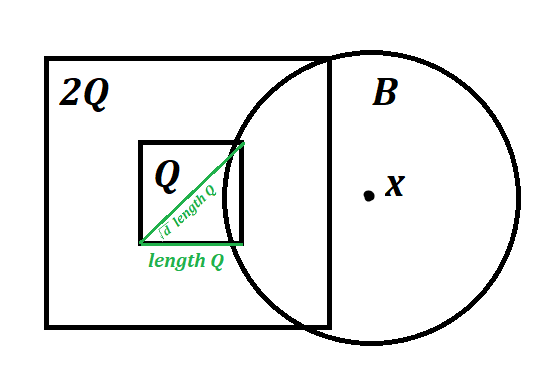
\includegraphics[scale = 0.5]{cubes}
	\end{center}
Since $b$ is supported in $\bigcup_k Q_k$, we can write
	\begin{align*}
		Mb_n (x)
			&= \sup_{r > 0} \frac{1}{|B_r (x)|} \int_{B_r (x)} |b_n (y)| \, dy = \sup_{r > 0} \frac{1}{|B_r (x)|} \sum_k \int_{Q_k \cap B_r (x)} |b_n (y)| \, dy \\
			&\lesssim \sup_{r > 0} \frac{1}{|B_{r (1 + 2 \sqrt d)} (x)|} \int_{B_{r (1 + 2 \sqrt d)} (x)}  \sum_k \mathbb 1_{Q_k} (z) \left( \frac{1}{|Q_k|} \int_{Q_k} |b_n (y)| \, dy \right) dz \leq \overline M b^{\text{ave}}_n (x),
	\end{align*}	
	for every $n$. This proves the claim, concluding the proof. 
\end{proof}

\subsection{The case $p \geq q$}

To complete the analogy with Calderon-Zygmund operators, we need a self-adjointness-type result for the maximal operator. This takes the form of a weighted maximal inequality. 

\begin{theorem}[Weighted maximal inequality]
	Let $\omega : \R^d \to [0, \infty)$ be a weight and $1 < p \leq \infty$, then the maximal operator $M$ satisfies the bounds
		\[ ||Mf||_{L^{1, \infty} (\omega dx)} \lesssim ||f||_{L^1 (M\omega dx)}, \qquad ||Mf||_{L^p (\omega dx)} \lesssim ||f||_{L^p (M \omega dx)} \]
	for scalar-valued $f : \R^d \to \C$. 
\end{theorem}

\begin{proof}
	Appealing to Marcinkiewicz interpolation, the strong-type $(p, p)$ inequality holds provided we show the weak-type $(1, 1)$ inequality and strong-type $(\infty, \infty)$ inequality. The latter follows from the usual strong-type $(\infty, \infty)$ inequality, remarking that $\omega dx \ll dx$ and $M\omega dx \ll dx$ and $dx \ll M\omega dx$. 
	
	It remains to show the weak-type $(1, 1)$ inequality. Let $K \subseteq \R^d$ be a compact subset satisfying
		\[ K \subseteq \{ x \in \R^d : Mf(x) > \lambda \}. \]
	We claim that 
		\[ \omega(K) \lesssim \frac1\lambda ||f||_{L^1 (M\omega dx)}. \]
	The weak-type $(1, 1)$ inequality follows immediately from inner regularity of $\omega dx$ and monotone convergence. By construction, for every $x \in K$ there exists $r(x) > 0$ such that 
		\begin{equation}
			 |B_{r(x)} (x)| \leq \frac1\lambda \int_{B_{r(x)} (x)} |f(y)| \, dy. 
			 \tag{*}
			\label{ineq:weighted} 
		\end{equation}	 	
	The collection $\{ B_{r(x)} (x) \}_{x}$ forms a cover of $K$, so we use compactness to extract a finite sub-cover, and the Vitali-Wiener covering lemma to extract a sub-collection of disjoint balls $B_{r_j} (x_j)$ satisfying $K \subseteq \bigcup_j B_{3r_j} (x_j)$. In place of the scaling property of the Lebesgue measure, we control the measure on the scaled balls with respect to $\omega$ by the maximal function of $\omega$. Note $B_{3r_j} (x_j) \subseteq B_{4r_j} (z)$ any $z \in B_{r_j} (x_j)$, so 
		\[ \omega(B_{3r_j} (x_j)) \leq \int_{B_{4r_j} (z)} \omega (y) \, dy \leq |B_{4r_j} (z)| \, M\omega(z). \]
	Integrating both sides against $|f|$ on the ball $B_{r_j} (x_j)$, we obtain	
		\begin{align*}
			 \omega(B_{3r_j} (x)) \int_{B_{r_j}(x_j)} |f(y)| \, dy 
			 	&\leq |B_{4 r_j} (z)| \int_{B_{r_j} (x_j)} |f(z)| \, M\omega (z) \, dz \\
			 	&\lesssim_d \frac1\lambda \left( \int_{B_{r_j} (x_j)} |f(y)| \, dy \right) \left( \int_{B_{r_j} (x_j)} |f(z)| \, M\omega (z) \, dz\right),
		\end{align*}	 
	where the second inequality follows from $|B_{4r_j} (z)| \sim |B_{r_j} (x_j)|$ and (\ref{ineq:weighted}). We conclude
		\[
			\omega(K)
				\leq\sum_j \omega(B_{3r_j} (x_j)) \lesssim_d \frac1\lambda \sum_j \int_{B_{r_j} (x_j)} |f(z)| \, M\omega (z) \, dz \leq \frac1\lambda ||f||_{L^1 (M\omega dz)}
		\]
	as desired. 
\end{proof}

\begin{remark}
	If $\omega \equiv 1$ then $M\omega \equiv 1$ and we recover the classical Hardy-Littlewood maximal inequality. For the theorem to be non-vacuous, we need the maximal function $M\omega$ to be finite a.e. This occurs precisely when 
		\[ \sup_{r \gg 1} \frac{1}{r^d} \int_{|y| \leq r} \omega(y) \, dy \lesssim 1. \]
	Assume the above holds, then $M\omega(x_0) < \infty$ for any Lebesgue point for $\omega$. Indeed, the averages of $\omega$ on small balls are controlled by Lebesgue differentiation theorem, while averages on large balls are controlled by the condition above
		\begin{align*}
			\frac{1}{|B_r (x_0)|} \int_{B_r (x_0)} \omega(y) \, dy \leq\frac{1}{|B_r (x_0)|} \int_{|y| \leq |x_0| + r} \omega(y) \, dy \lesssim \frac{|B_{|x_0| + r} (0)|}{|B_r (x_0)|} \frac{1}{(|x_0| + r)^d} \int_{|y| \leq |x_0| + r} \omega(y) \, dy \lesssim 1
		\end{align*}
	for $r \gg 1$. This shows that $M\omega(x_0) < \infty$. Conversely, suppose $M\omega(x_0) < \infty$, then 
	\begin{align*}
		\frac{1}{r^d} \int_{|y| \leq r} \omega(y) \, dy \leq \frac{1}{r^d} \int_{B_{|x_0| + r} (x_0)} \omega(y) \, dy \lesssim \frac{(|x_0| + r)^d}{r^d} (M\omega)(x_0) \lesssim 1
	\end{align*}
	for $r \geq |x_0|$ uniformly. 
\end{remark}

\begin{proof}[Proof of Theorem \ref{thm:vectorvalued} for $p \geq q$]
	Observe that $1 < (p/q)' \leq \infty$. By duality we can write
	\begin{align*}
		||\overline M_q f||_{L^p}^q
			&= || |\overline M_q f|^q ||_{L^{p/q}} = \sup_{||\omega||_{L^{(p/q)'}} \leq 1}\int_{\R^d} |\overline M_q f (x)|^q \omega(x) \, dx =\sup_{||\omega||_{L^{(p/q)'}} \leq 1} \sum_{n \in \N}  \int_{\R^d} |Mf_n (x)|^q \omega(x) \, dx \\
			&\lesssim \sup_{||\omega||_{L^{(p/q)'}} \leq 1} \sum_{n \in \N}  \int_{\R^d} |f_n (x)|^q M \omega(x) \, dx = \sup_{||\omega||_{L^{(p/q)'}} = 1} \int_{\R^d} |f(x)|^q M\omega (x) \, dx \\
			&\lesssim \sup_{||\omega||_{L^{(p/q)'}} \leq 1} || |f|^q||_{L^{p/q}} ||M\omega||_{L^{(p/q)'}} \\
			&\lesssim \sup_{||\omega||_{L^{(p/q)'}} \leq 1} || |f|^q||_{L^{p/q}} ||\omega||_{L^{(p/q)'}} \leq || f||_{L^p}^q,
	\end{align*}
where the first inequality follows from the weighted maximal inequality, the second from Holder's inequality, and the third from the strong-type $((p/q)', (p/q)')$ bound for the maximal operator. 
\end{proof}


\bibliographystyle{alpha}
\bibliography{biblio}

\end{document}